\makeatletter
\def\input@path{{../../}}
\makeatother
\documentclass[../../main.tex]{subfiles}

\graphicspath{
	{../../img/}
	{../img/}
	{img/}
}

\begin{document}
	
\begin{rems}

\;

\begin{enumerate}
	\item В обосновании достаточности доказанной теоремы существенную роль 
	играло предположение о непрерывности дифференцируемой функции 
	$ u = \Re f(z) $ и $ v = \Im f(z) $. В общем случае  можно отказаться 
	от него, но при условии этом доказательство значительно усложнится.
	\item Используя условие Коши-Римана \eqref{lec28:17}, из \eqref{lec28:21} 
	также имеем:
	\begin{equation}
	\label{lec29:22} 
	f'(z) = v_y' - iu_y' = \left[u_y' = -v_x'\right] =
	v_y' + iv_x' = \left[v_y' = u_x'\right] = u_x' + iv_x' = u_x' - iu_y'.
	\end{equation}
	\item Для $ \forall c, y \in \R $ рассмотрим 
	$ F(x, y) = f(x + iy) = u + iv,\ u, v \in \R $
	и, применяя правило дифференцирования сложных ФКП получаем, что 
	\[ 
	F_x' = (f(z))_x' = f'(z)z_x' = \left[
	\begin{gathered}
		z = x + iy\\
		z_x' = 1
	\end{gathered}
	\right] = f'(z) = (u + iv)_x' = u_x' + iv_x'.
	\]
	Аналогично
	\[ 
	F_y' = (f(z))_y' = f'(z)z_y' = \left[
	\begin{gathered}
	z = x + iy\\
	z_y' = i
	\end{gathered}
	\right] = if'(z) = i(u_x' + iv_x').\]
	Также выполняется $F_y' = u_y' + iv_y'$, откуда получаем
	\[u_y' + iv_y' = i(u_x' + iv_x') \implies -v_x' + iu_x' = u_y' + iv_y' 
	\implies \eqref{lec28:17}.\]
	Указанные действия поясняют смысл условий Коши-Римана \eqref{lec28:17}.
\end{enumerate}
\end{rems}
\begin{exmps}

\;

\begin{enumerate}
	\item $ f(z) = z = x + iy,\ x, y \in \R $
	\[
	\begin{cases}
		u = \Re f(z) = x,\\
		v = \Im f(z) = y.
	\end{cases}
	\]
	Имеем 
	\[
	\begin{cases}
		u_x' = 1 = v_y',\\
		u_y' = 0 = -v_x'.
	\end{cases}
	\]
	Условия \eqref{lec28:17} выполняются, значит, ФКП является дифференцируемой,
	причём $ f'(z) = (z)' \stackrel{\eqref{lec28:21}}{=} u_x' + iv_x' = 
	1 + i\cdot0 = 1 $, что согласуется с действительным случаем.
	\item $ f(z) = \overline{z} = x - iy,\ x, y \in \R $.
	
	$ u = x,\ v = -y, \implies u_x' = 1 \neq -1 = v_y' $. 
	Условие Коши-Римана не выполняется $ \implies $ ФКП 
	не дифференцируема ни в одной точке.
	\item $ f(z) = z \Re z = x(x + iy) $
	\[
	\begin{cases}
		u = \Re f(z) = x^2,\\
		v = \Im f(z) = xy.
	\end{cases}
	\]
	Проверим выполнение \eqref{lec28:17}:
	\[
	\begin{cases}
		u_x' = 2x = x = v_y'\\
		u_y' = 0 = -y = -v_x'
	\end{cases} \implies
	\begin{cases}
		x = 0\\
		y = 0
	\end{cases}
	\]
	Значит, рассматриваемая функция дифференцируема только в точке
	$ z_0 = (0, 0) $. Причём
	$ f'(0) = u_x'(0, 0) + iv_x'(0, 0) = 0 $.
	\item $ f(z) = e^z = e^{x + iy} = e^x(\cos y + i\sin y),\ x, y \in \R $.
	\[
	\begin{cases}
		u = \Re f(z) = e^x \cos y,\\
		v = \Im f(z) = e^x \sin y.
	\end{cases}
	\]
	Опять составим \eqref{lec28:17}:
	\[
	\begin{cases}
	u_x' = e^x \cos y = e^x \cos y = v_y',\\
	u_y' = -e^x \sin y = -e^x \sin y = -v_x'.
	\end{cases}
	\]
	Условие \eqref{lec28:17} выполнено для $ \forall z \in \C $, 
	поэтому комплексная экспонента является дифференцируемой функцией в $ \C 
	$, причём
	\[
	f'(z) = (e^z)' = u_x' + iv_x' = e^x \cos y + ie^x \sin y =
	e^x(\cos y + i\sin y) = e^{x + iy} = e^z,
	\]
	что также согласуется с производной действительной экспоненты.
\end{enumerate}
\end{exmps}

Аналогичным образом находят производные основных элементарных ФКП, 
и при этом получаемые формулы будут естественным образом обобщаться для
соответствующих элементарных действительных функций. Например:
\[
\begin{gathered}
(\sin z)' = \cos z,\\ (\cos z)' = -\sin z,\\
(\tg z)' = \dfrac{1}{\cos^2 z},\\ 
(\ctg z)' = -\dfrac{1}{\sin^2 z},\\
(\Ln z)' = \dfrac{1}{z},\\
(\Arcsin z)' = \dfrac{1}{\sqrt{1 - z^2}},\\
(\Arccos z)' = -\dfrac{1}{\sqrt{1 - z^2}},\\
(\Arctg z)' = \dfrac{1}{1 + z^2},\\
(\Arcctg z)' = -\dfrac{1}{1 + z^2}.
\end{gathered}
\]
\begin{exc}
	Записать соответствующие формулы для гиперболических 
	и обратных к ним функций.
\end{exc}
\begin{eans}
\begin{gather*}
(\sh z)' = \ch z,\\
(\ch z)' = \sh z,\\
(\th z)' = \dfrac{1}{\ch^2 z},\\
(\cth z)' = -\dfrac{1}{\sh^2 z},\\
(\Arsh z)' = \dfrac{1}{\sqrt{z^2 + 1}},\\
(\Arch z)' = \dfrac{1}{\sqrt{z^2 - 1}},\\
(\Arth z)' = \dfrac{1}{1 - z^2},\\
(\Arcth z)' = \dfrac{1}{1 - z^2}.
\end{gather*}
\end{eans}

\section{Гармонические функции}

Как будет получено позже, если ФКП $ f(z) $ дифференцируема в области
$ D \subset \C $, т.~е. $ \forall z \in D \quad\exists f'(z) \in \C $, то она 
будет,
в отличие от вещественных функций, бесконечное число раз дифференцируема в 
$D$. Поэтому действительные функции 
\[
\begin{cases}
	u = u(x, y) = \Re f(z),\\
	v = v(x, y) = \Im f(z)
\end{cases}
\]
будут также бесконечное число раз дифференцируемы. Отсюда, используя условие
Коши-Римана \eqref{lec28:17} следует:
\[
\begin{gathered}
\exists u_{x^2}'' = (u_x')_x' 
\stackrel{\eqref{lec28:17}}{=}
[u_x' = v_y'] = (v_y')_x' = v_{yx}''\\
\exists u_{y^2}'' = (u_y')_y' 
\stackrel{\eqref{lec28:17}}{=}
[u_y' = -v_x'] = (-v_x')_y' = -v_{yx}''\\
\end{gathered}
\]
Из теоремы о равенстве смешанных производных Ф2П следует, что 
$ u_{xy}'' = v_{xy}'' $. Поэтому $ u_{x^2}'' + u_{y^2}'' = v_{xy}'' - 
v_{xy}'' = 0 $.

Аналогично показывается, что $ v_{x^2}'' + v_{y^2}'' = \dots = 0 $.

Введем \emph{дифференциальный оператор Лапласа}:
\[
\D = \dfrac{d^2 (.)}{d x^2} + \dfrac{d^2(.)}{d y^2}
\]
Для дважды дифференцируемой $ F = F(x, y) $ имеем\[
\D F = \dfrac{d^2 F}{d x^2} + \dfrac{d^2 F}{d y^2} = 
F_{x^2}'' + F_{y^2}''.
\]
В общем случае, если дважды дифференцируемая Ф2П $ F(x, y) $
удовлетворяет $ \D F = 0 $, то эта Ф2П называется \emph{гармонической 
функцией}.
Из сказанного выше следует, что действительная и мнимая части 
дифференцируемой ФКП являются гармоничесими функциями, т.~е.
$ \D u = 0$ и $\D v = 0 $.

Произвольная пара функций $ u = u(x, y),\ v = v(x, y) $, где $u$ и $v$~--- 
гармонические и 
удовлетворяют условиям Коши-Римана \eqref{lec28:17},
называется \emph{сопряжённой парой гармонических функций}.

Можно показать, что любую дифференцируемую ФКП можно восстановить с точностью 
до константы, зная лишь её действительную или мнимую часть.
\begin{exmp}
Найдём дифференцируемую ФКП $ f(z) = u + iv,\ u, v\in \R $,
если \[\begin{cases}u = \Re f(z) = 2xy, \\ f(1 + i) = 2. \end{cases}\]
Проверим корректность постановки:
\begin{enumerate}
	\item[а)] $ u $~--- гармоническая функция.
	\[\D u = u_{x^2}'' + u_{y^2}'' = (2y)_x' + (2x)_y' = 0. \]
	\item[б)] \[
	\begin{cases}
		z_0 = 1 + i = x_0 + iy_0,\\
		x_0 = 1,\ y_0 = 1,
	\end{cases}
	f(1 + i) = u(x_0, y_0) + iv(x_0, y_0) = \left[
	\begin{gathered}
		u(1, 1) = 2\cdot1\cdot1 = 2\\
		v(1, 1) = 0
	\end{gathered}
	\right] = 2.
	\]
	Для восстановления требуется найти $ v(x, y) $.
	
	Из равенств выше получаем, что $ v(1, 1) = 0 $.
	Т.~к. $ u, v $~--- комплексно-сопряжённая пара
	гармонических функций, то в силу \eqref{lec28:17} имеем
	\[
	\begin{cases}
		v_x' = -u_y' = -2x,\\
		v_y' = u_x' = 2y.
	\end{cases}
	\]
	Используя неопределенные интегралы, получаем \[ 
	v = -2\int x dx = -x^2 + C(y) 
	\implies v_y' = C'(y) = 2y \implies 
	C(y) = 2\int y dy = y^2 + C \implies \]\[ \implies
	v(x, y) = -x^2 + y^2 + C.
	\]
	Используя $ v(1, 1) = 0$ получаем:
	\[v(1, 1) = -1 + 1 + C = 0 \implies C = 0 \implies 
	v(x, y) = y^2 - x^2.\]
	Значит, \[ f(z) = u + iv = 2xy + i(y^2 - x^2) =
	-i(2ixy - y^2 + x^2) = -i(x + iy)^2 = -iz^2.\]
\end{enumerate}
\end{exmp}

\section{Геометрический смысл модуля и производной аналитической ФКП}

Далее дифференцируемую в каждой точке $ D $ ФКП $ f(z) $
будем называть \emph{аналитической} в $ D $.

Пусть $ f(z) $~--- аналитическая в некоторой окрестности $ z_0 \in D $ и 
$ f'(z_0) \neq 0 $. Тогда
\[
f'(z_0) = k e^{i\phi},\
\begin{cases}
	k = \abs{f'(z_0)} > 0,\\
	\phi = \arg f'(z_0) \in \left]-\pi; \pi\right].
\end{cases}
\]
Придадим $ z_0 \in D $ достаточно малое произвольное приращение 
$ \D z \in \C $ так, чтобы $ z_0 + \D z $ лежало в 
окрестности
дифференцируемости $ f(z) $. Тогда для $w = f(z)$ получаем, что
\[\exists \lim\limits_{\D z \to 0} \dfrac{\D w(z_0)}{\D z} = f'(z_0).\]
Отсюда для достаточно малых приращений получаем
\[
\abs{\dfrac{\D w(z_0)}{\D z}} \approx \abs{f'(z_0)} = k > 0
\implies \abs{\D w(z_0)} \approx k\abs{\D z}.
\]
Для $ \phi = \arg f'(z_0) $ получаем: \[ \phi \approx \arg 
\dfrac{\D w(z_0)}{\D z} = \arg \D w(z_0) - \arg \D z \implies
\alpha = \arg \D w(z_0) \approx \phi + \arg \D z.
\]
Т.~е.
\begin{equation}
\label{lec29:23}
\begin{cases}
	\abs{\D w (z_0)} \approx k\abs{\D z},\\
	\arg \D w(z_0) \approx \phi + \arg \D z.
\end{cases}
\end{equation}
Получаем, что производная ФКП имеет следующий геометрический смысл:

\begin{center}
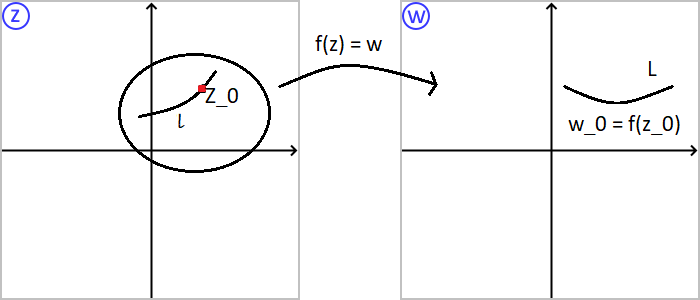
\includegraphics{lec29_1}
\end{center}

Первое из равенств в \eqref{lec29:23}, с учётом того, что модуль комплексного 
числа
есть длина радиус-вектора соответствующей точки, говорит о том, что в 
достаточно 
малых окрестностях точки $ z_0 $ длины образа $ L $ и прообраза $ l $ связаны 
соотношением:
$\text{Длина $L$} \approx k \cdot \text{Длина $l$}$. 
Поэтому если $ k = \abs{f'(z_0)} > 1 $, то имеем растяжение длин, 
а если $ 0 < k < 1 $~--- сжатие.
Далее, изобразим $ l $ и $ L $ на совмещённом чертеже, где 
$ z_0 $ и $ w_0 $ совпадают. Для касательных к этим 
линиям в совмещённой точке имеем:
\begin{center}
	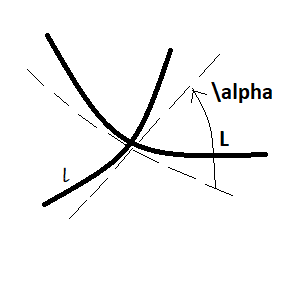
\includegraphics{lec29_2}
	\begin{gather*}
	\alpha \approx \arg \D w(z_0) \approx \phi + \arg \D z
	\text{~--- получаем поворот на угол $\alpha$.}
	\end{gather*}
\end{center}
Это является геометрическим смыслом аргумента $f$.

Далее отображение $ f(z) = w $ (необязательно дифференцируемое), которое
в каждой точке $ z_0 \in D $ сохраняет постоянное растяжение
и поворот, будем называть \emph{конформным}.
Если при этом ориентация образа сохраняется, то такое конформное отображение
называется отображением I рода, иначе~--- II рода.

Можно показать, что если $ w = f(z) $~--- конформное отображение I рода, 
то $ w = \overline{f(z)} $ будет конформным отображением II рода.

Используя геометрический смысл модуля производной аналитической ФКП,
можно показать, что если в $ D \subset \C $ имеется гладкая линия
$ l \subset D $, заданная параметрически: \[
\begin{cases}
 z = x(t) + iy(t),\\
 t_1 \leq t \leq t_2,
\end{cases}
\]
то тогда
для $ L = f(l) $~--- образа $ l $ при аналитическом отображении $ w = f(z) $,
имеем:
\begin{equation}
\label{lec30:1}
\text{Длина } L = \int\limits_{l} \abs{f'(z)} \abs{dz}.
% Было:
% 
% \text{Длина } L = \int\limits_{l} \abs{f'(z(t))} dt = 
% \int\limits_{l} \sqrt{(x'(t))^2 + (y'(t))^2} \; dt.
\end{equation}

Аналогично, если рассматривается квадратная область $ G \subset D $, 
то для площади $ G $ получаем следующее. Пусть $S$~--- площадь $f(G)$~--- 
образа $G$ при аналитическом отображении $ w = f(z) $. Тогда
\begin{equation}
\label{lec30:2}
S = \iint\limits_{G} \abs{f'(z)}^2 dx\;dy.
\end{equation}

\end{document}
